\documentclass[border=8pt]{standalone}
\usepackage[T1]{fontenc}
\usepackage[utf8]{inputenc}
\usepackage{tikz}
\usetikzlibrary{shapes.multipart,arrows.meta,positioning}
\tikzset{
  clase/.style={draw,rectangle split,rectangle split parts=3,align=left,font=\scriptsize\ttfamily,inner sep=3pt},
  her/.style={-{Triangle[open,length=3mm]}},
  comp/.style={{Diamond[fill=black,length=3.5mm]}-},
  agr/.style={{Diamond[open,length=3.5mm]}-},
  dep/.style={dashed,-{Straight Barb}},
  aso/.style={-{Straight Barb}},
  m/.style={font=\scriptsize}}
\newcommand{\cl}[3]{\textbf{#1}\nodepart{second}#2\nodepart{third}#3}
\begin{document}
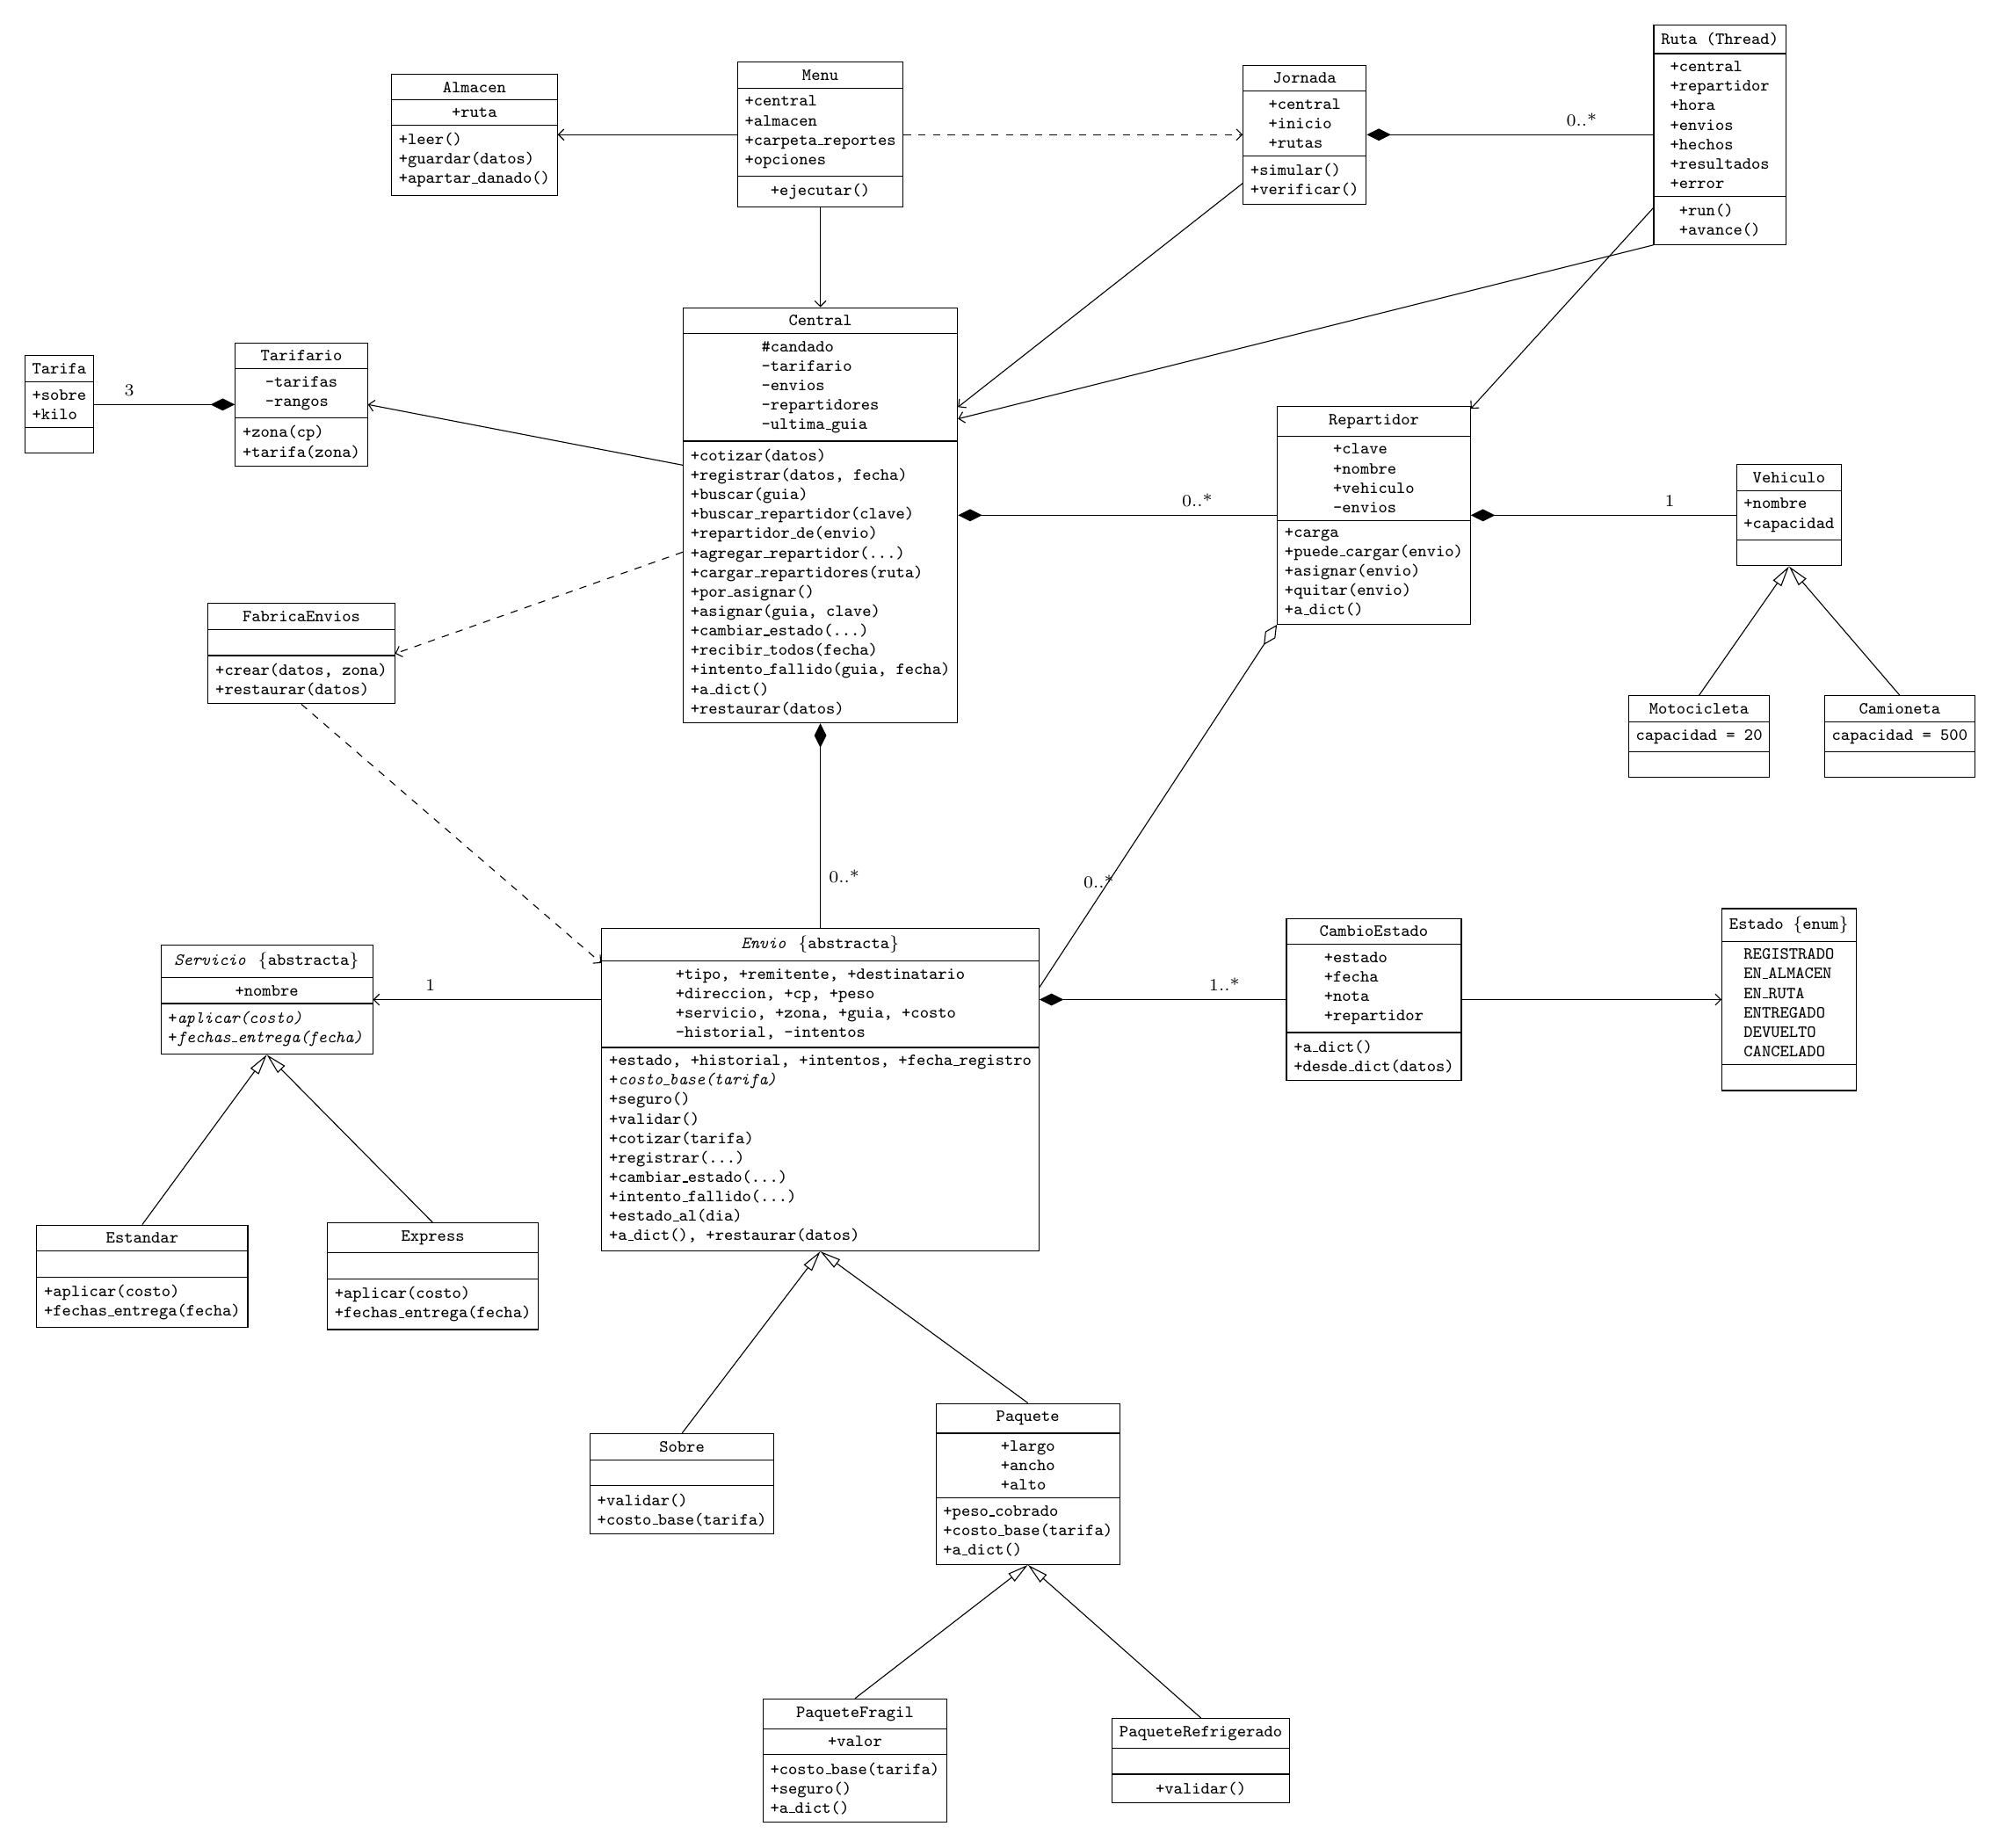
\begin{tikzpicture}
\node[clase] (menu) at (0,9.5) {\cl{Menu}{+central\\+almacen\\+carpeta\_reportes\\+opciones}{+ejecutar()}};
\node[clase] (alm) at (-5,9.5) {\cl{Almacen}{+ruta}{+leer()\\+guardar(datos)\\+apartar\_danado()}};
\node[clase] (cen) at (0,4) {\cl{Central}{\#candado\\-tarifario\\-envios\\-repartidores\\-ultima\_guia}{+cotizar(datos)\\+registrar(datos, fecha)\\+buscar(guia)\\+buscar\_repartidor(clave)\\+repartidor\_de(envio)\\+agregar\_repartidor(...)\\+cargar\_repartidores(ruta)\\+por\_asignar()\\+asignar(guia, clave)\\+cambiar\_estado(...)\\+recibir\_todos(fecha)\\+intento\_fallido(guia, fecha)\\+a\_dict()\\+restaurar(datos)}};
\node[clase] (tar) at (-7.5,5.6) {\cl{Tarifario}{-tarifas\\-rangos}{+zona(cp)\\+tarifa(zona)}};
\node[clase] (ta) at (-11,5.6) {\cl{Tarifa}{+sobre\\+kilo}{}};
\node[clase] (fab) at (-7.5,2) {\cl{FabricaEnvios}{}{+crear(datos, zona)\\+restaurar(datos)}};
\node[clase] (jor) at (7,9.5) {\cl{Jornada}{+central\\+inicio\\+rutas}{+simular()\\+verificar()}};
\node[clase] (rut) at (13,9.5) {\cl{Ruta (Thread)}{+central\\+repartidor\\+hora\\+envios\\+hechos\\+resultados\\+error}{+run()\\+avance()}};
\node[clase] (rep) at (8,4) {\cl{Repartidor}{+clave\\+nombre\\+vehiculo\\-envios}{+carga\\+puede\_cargar(envio)\\+asignar(envio)\\+quitar(envio)\\+a\_dict()}};
\node[clase] (veh) at (14,4) {\cl{Vehiculo}{+nombre\\+capacidad}{}};
\node[clase] (mot) at (12.7,0.8) {\cl{Motocicleta}{capacidad = 20}{}};
\node[clase] (cam) at (15.6,0.8) {\cl{Camioneta}{capacidad = 500}{}};
\node[clase] (env) at (0,-4.3) {\cl{\textit{Envio} \{abstracta\}}{+tipo, +remitente, +destinatario\\+direccion, +cp, +peso\\+servicio, +zona, +guia, +costo\\-historial, -intentos}{+estado, +historial, +intentos, +fecha\_registro\\+\textit{costo\_base(tarifa)}\\+seguro()\\+validar()\\+cotizar(tarifa)\\+registrar(...)\\+cambiar\_estado(...)\\+intento\_fallido(...)\\+estado\_al(dia)\\+a\_dict(), +restaurar(datos)}};
\node[clase] (cam2) at (8,-3) {\cl{CambioEstado}{+estado\\+fecha\\+nota\\+repartidor}{+a\_dict()\\+desde\_dict(datos)}};
\node[clase] (est) at (14,-3) {\cl{Estado \{enum\}}{REGISTRADO\\EN\_ALMACEN\\EN\_RUTA\\ENTREGADO\\DEVUELTO\\CANCELADO}{}};
\node[clase] (ser) at (-8,-3) {\cl{\textit{Servicio} \{abstracta\}}{+nombre}{+\textit{aplicar(costo)}\\+\textit{fechas\_entrega(fecha)}}};
\node[clase] (sta) at (-9.8,-7) {\cl{Estandar}{}{+aplicar(costo)\\+fechas\_entrega(fecha)}};
\node[clase] (exp) at (-5.6,-7) {\cl{Express}{}{+aplicar(costo)\\+fechas\_entrega(fecha)}};
\node[clase] (sob) at (-2,-10) {\cl{Sobre}{}{+validar()\\+costo\_base(tarifa)}};
\node[clase] (paq) at (3,-10) {\cl{Paquete}{+largo\\+ancho\\+alto}{+peso\_cobrado\\+costo\_base(tarifa)\\+a\_dict()}};
\node[clase] (fra) at (0.5,-14) {\cl{PaqueteFragil}{+valor}{+costo\_base(tarifa)\\+seguro()\\+a\_dict()}};
\node[clase] (ref) at (5.5,-14) {\cl{PaqueteRefrigerado}{}{+validar()}};
\draw[aso] (menu) -- (cen);
\draw[aso] (menu) -- (alm);
\draw[dep] (menu) -- (jor);
\draw[aso] (jor) -- (cen);
\draw[comp] (jor) -- node[m,near end,above]{0..*} (rut);
\draw[aso] (rut) -- (rep);
\draw[aso] (rut.south west) -- (cen.35);
\draw[aso] (cen.160) -- (tar.east);
\draw[comp] (tar) -- node[m,near end,above]{3} (ta);
\draw[dep] (cen.195) -- (fab.east);
\draw[dep] (fab.south) -- (env.150);
\draw[comp] (cen) -- node[m,near end,right]{0..*} (env);
\draw[comp] (cen) -- node[m,near end,above]{0..*} (rep);
\draw[comp] (rep) -- node[m,near end,above]{1} (veh);
\draw[agr] (rep.south west) -- node[m,near end,above]{0..*} (env.25);
\draw[her] (mot.north) -- (veh.south);
\draw[her] (cam.north) -- (veh.south);
\draw[comp] (env.east |- cam2.west) -- node[m,near end,above]{1..*} (cam2.west);
\draw[aso] (cam2) -- (est);
\draw[aso] (env.west |- ser.east) -- node[m,near end,above]{1} (ser.east);
\draw[her] (sta.north) -- (ser.south);
\draw[her] (exp.north) -- (ser.south);
\draw[her] (sob.north) -- (env.south);
\draw[her] (paq.north) -- (env.south);
\draw[her] (fra.north) -- (paq.south);
\draw[her] (ref.north) -- (paq.south);
\end{tikzpicture}
\end{document}
